% THIS IS SIGPROC-SP.TEX - VERSION 3.1
% WORKS WITH V3.2SP OF ACM_PROC_ARTICLE-SP.CLS
% APRIL 2009
%
% It is an example file showing how to use the 'acm_proc_article-sp.cls' V3.2SP
% LaTeX2e document class file for Conference Proceedings submissions.
% ----------------------------------------------------------------------------------------------------------------
% This .tex file (and associated .cls V3.2SP) *DOES NOT* produce:
%       1) The Permission Statement
%       2) The Conference (location) Info information
%       3) The Copyright Line with ACM data
%       4) Page numbering
% ---------------------------------------------------------------------------------------------------------------
% It is an example which *does* use the .bib file (from which the .bbl file
% is produced).
% REMEMBER HOWEVER: After having produced the .bbl file,
% and prior to final submission,
% you need to 'insert'  your .bbl file into your source .tex file so as to provide
% ONE 'self-contained' source file.
%
% Questions regarding SIGS should be sent to
% Adrienne Griscti ---> griscti@acm.org
%
% Questions/suggestions regarding the guidelines, .tex and .cls files, etc. to
% Gerald Murray ---> murray@hq.acm.org
%
% For tracking purposes - this is V3.1SP - APRIL 2009

\documentclass{acm_proc_article-sp}

\begin{document}



\title{Catchy Part: Surveying Users' Perceptions of Threats for Wearable Devices}
%\titlenote{(Does NOT produce the permission block, copyright information nor page numbering). For use with ACM\_PROC\_ARTICLE-SP.CLS. Supported by ACM.}}

%\subtitle{[Extended Abstract]
%\titlenote{Note
%\textit{Note \LaTeX$2_\epsilon$\ and BibTeX} at \texttt{www.website.com}}}


\numberofauthors{3} 

\author{
% 1st. author
\alignauthor
Linda N. Lee\\
       \affaddr{UC Berkeley}\\
       \email{lnl@cs.berkeley.edu}
% 2nd. author
\alignauthor
Serge Egelman\\
       \affaddr{UC Berkeley}\\
       \affaddr{ICSI}\\
       \email{serge@cs.berkeley.edu}
% 3rd. author
\alignauthor David Wagner\\
       \affaddr{UC Berkeley}\\
       \email{daw@cs.berkeley.edu}
}

\maketitle



\begin{abstract}
(Okay, kind of intimidated with writing the abstract. My plan is to write intro/conclusion first and then condense it into here, while nodding off to the contributions that we made.) At the very least, I can say that we studied user perceptions for threats in wearable devices, along with user perceptions of risk and benefit for emerging technologies and what they thought was the biggest risk for using wearable devices. Data type, data recipient, and device type all matter different amounts. All new technologies were perceived to be low risk low benefit but we think this is because people are unfamiliar with these technologies. Privacy was the number one concern, followed by security, then health, money, social norms changing and social stigma. Fantastic ending sentence here.
\end{abstract}

% A category with the (minimum) three required fields
\category{look it up}{keyword1}{keyword2}{keyword3}
%A category including the fourth, optional field follows...
%\category{D.2.8}{Software Engineering}{Metrics}[complexity measures, performance measures]

\terms{term1} {term2} {term3}

\keywords{Privacy, Security, User Studies, Risk Perception, Ubiquitous Computing, Wearables} % NOT required for Proceedings

%%%%%%%%%%%%%%%%%%%
%%%         PAPER BODY         %%%
%%%%%%%%%%%%%%%%%%%

\section{Introduction}
(REDO) Basically a longer version of the abstract, plus some additional motivational things thrown in here. I feel like I should have a couple sentences which lead into what I am going to talk about, or at least lead in with something catchy and strong. Hmm. Think about what to put here.

A huge paragraph or two on why wearables are important and how much they are in use. Basically, prove that the study is worth doing in the first place. Some sources to use: 2014 is year of wearables \cite{Forbes}. A survey consisting of 3,956 respondents who are either current users or non-users with high interest in wearables \cite{Neilsen} says that most popular devices (61\%), followed by smart watches (45\%) and mHealth (mobile health) devices (17\%). It is estimated that ~15\% use it in daily life \cite{Nilsen}\cite{WearableStatNews}.

People are getting upset and scared about the things that can happen with wearble devices. There was a scandal with fitbit where the 1) profiles were default public and 2) sex counted as an exercise (cite that), how google had to disable facial recognition for glass (cite) along with using voice commands rather than other commands for bystanders to be informed of what is going on (cite). We suspect that there will only be more and more situations like this to come, as wearables get increasingly powerful (cite) and are getting adopted by more people (cite), and across other demographics (cite). 

End this section with an explicit list of contributions made by this paper. \\[-.8cm]

\begin{itemize} \itemsep1pt \parskip0pt \parsep0pt
\item we got people's perception on various new threats for wearable devices, a wide range of threats.
\item we found out what matters in their perception of these things--data type, data recipient, and device type and how much each of those matter. We have a cool regression model for that. 
\item we found out how people's perception of threats change when it is with respect to other people consuming the data, or just the device (data type analysis ranking with appserver only verse everyone else). 
\item we got people's risk and benefit assessment of new technologies and capabilities. Most new capabilities are seen as low risk low benefit, but we suspect it's because people aren't familiar. 
\item we found out what people were, nebulously, most concerned with. Privacy, then security, health, finances, social norms. 
\item we calibrate our work so it's relevant and understandable with smartphone research and risk perception research. We can even say that we extended those areas too, if I want to be bold. 
\end{itemize}

%%%%%%%%%%%%%%%%%%%

\section{Related Work}
In this paper, we explore user perceptions of security threats for wearable devices. In this section, we discuss related works which explore threats for smartphones and wearable devices, discuss emerging challenges related to ubiquitous computing, and study user perceptions of threats and technologies. 

\subsection{Concerns for Smartphones and Wearables}
(REDO) Mention Adrienne's work here, and other relevant smartphone studies of any sort. I will talk about how I model Adrienne's work in the next section, Survey, just give a nod to it here and go into it later. Since my results were that people care about privacy, security, health, and social change/social stigma, any phone studies which hint at any of those things will be good to put here. Be sure to go cite a fair number of them. Related work section is the part where it looks like I know stuff. 

Mention any studies for wearables (like the ones you can find at Ubicomp, CHI, or SOUPS), and give them a nod. Especially mention ones on privacy and perceptions, since I know those exist. I doubt there will be ones for social norm shifts/social stigma, or health concerns, but maybe I can at least include some security ones here too. Throughout mentioning all of these works, highlight how my study is different from previous studies. 

\subsection{Ubiquitous Computing}
(REDO) As technology becomes more and more ubiquitous, more sensors will record more things about more people more of the time. There are an endless amount of unique situations which can negatively impact a person's privacy or security. There is a clear need to better communicate these risks to people (cite webcam paper and other papers here?), but there are too many things to warn people about. Therefore, we need to know what are the most threatening and also most relevant situations to inform the users about, since we can't bug them all the time about everything. 

We need to investigate the threat landscape and people's privacy concerns now, before wearables are widely adopted, or designed without these considerations in mind. So although our research is at at time when things are rapidly changing and most people don't have wearables, it is crucial to do the research now so we can prevent badness later.

\subsection{User Perception}
(REDO) In this paper, we investigate one of the two important questions--what are the most relevant situations to people. We do this firstly because people are really bad at knowing the likelihood of something, especially a threat with respect to security or privacy, is going to happen (sources here). And while the most damaging situations should also be addressed, this is not yet possible since these technologies haven't been adopted and the damage hasn't happened, so we don't know yet. Additionally, since the number one concern that people had with these devices was privacy (can I say result here? I guess I already did in abstract), we need to know what people consider private, which is more nuanced and requires a user study like this survey. 

We also study risk. Mention Fischoff here. This is a very seminal paper in risk perception and it also studies how safe enough something has to be before people can accept something. I will talk about how I model my work in the next section, Survey, just give it a nod here and go into it later. Also mention at least a couple more works related to risk perception here to round it off. 

%%%%%%%%%%%%%%%%%%%

\section{Survey}
The survey design process consisted of synthesizing a relevant and comprehensive set of questions, validating the relevance, clarity, and completeness of the questions, and concluded with finalizing distribution logistics. Details on the synthesis, validation, methodology, and data are below.

\subsection{Threat Landscape Investigation} 
(REDO) To generate the list of possible scenarios which can happen with a wearable device, we did three things. Firstly, we looked at the most popular list of wearable technologies (including the Fitbit fitness tracker, Pebble smartwatch, and Glass wearable computing device) and their sensors and capabilities. Secondly, we looked at past research in mobile devices and current wearable device considerations. Thirdly, we finished off brainstorming possible things yet to come by looking at vision videos for wearables, and the news for possible concerns. 

We already motivated why ubiquitous computing is relevant and we need to do it, so no need to do it here. In the end, we ended up focusing questions on new capabilities that wearables have that smartphones and other devices do not, existing sensors, any concerns which might infringe on security and privacy, along with a couple investigative ones (like if someone recorded all your conversations but never shared it, are you going to be upset? that might be taken out of this paper, but still). 

\subsection{Calibrating with Existing Works}
(REDO) Mobile devices threats are well studied and the closest well-researched thing to wearable device threats. We used the same format as Adrienne's paper so that we can compare our results to the ones that she got in her study for mobile devices. We purposed used the same scale and question format as she did in her study, but it's a pretty defensible scale to use anyway and the wording was about consistent with how we were going to do it anyway. Defend the likert scale use and the wording of the question a bit here. Because it is similar, and we also had calibrating questions, we can compare the threats with respect to existing threats studied. We're so relevant, yay. 

We used a prompt similar to Fischoff's study so that we could compare our results to the ones that he got in his study, and to put more of the new technologies onto the risk/benefit map. This way, we can have a sense of the risk and benefit with respect to well-studied and more familiar technologies. This also makes the results that we have more accurate and tangible, since people have anchors to base their assessments off of, rather than comparing a bunch of things that seem nebulous to them.

\subsection{Validation}
(REDO) We conducted a focus group to look over the list, brainstorm more scenarios,  and get question feedback. We got a small sample of results (which were guided so we through them out, but it was helpful to know what we might expect) and clarify any scenarios which were unclear. Logistically, we also used this time to time the survey, made sure the survey worked, and other things. Quick demographics of the focus group here--(fix later) 12 people, X\% male, average age Y, with education ranging from A to B and professions including student, artist, business person, court judge, etc.  You can look at the focus group script in appendix \ref{sec:script}.

\subsection{Methodology}
We recruited 2,250 participants August 7th-13th 2014 via Amazon's Mechanical Turk. We restricted participants to those over 18 years old. No other restrictions on participation were applier. We asked questions regarding participants' perceptions of various situations which might occur when wearing a wearable device, and about the risks and benefits of new technologies.
 
 %%%%%%%%%%%%%%%%%%%
 
\section{Questions}
The survey consisted of questions regarding concerns with respect to a factious wearable device called the Cubetastic3000 (this was done to prevent any biases in answers from participants with respect to specific companies), smartphone concerns, risk and benefit assessment of technologies, and exit questions. Details on the question ordering, question formatting, and sample questions are below. The full survey can be found at http://www.surveygizmo.com/s3/1657924 /Wearables-Threats-User-Survey. 

\subsection{Format}
(REDO) In total, the survey consisted of 367 unique questions, with each participant answering 27 questions. Out of the 27 seen by the participant, 10 of the questions are randomly selected from a particular set of questions (see below).   \\[-.8cm]

\begin{itemize} \itemsep1pt \parskip0pt \parsep0pt
\item 2 comprehension questions 
\item 6/305 questions about various scenarios 
\item 2/5 questions about smartphone scenarios 
\item 1/20 benefit questions 
\item 1/20 risk questions (same technology) 
\item 4 demographics
\item 1 open-ended question 
\item 10 questions of IUIPC \\[-.8cm]
\end{itemize}

To mitigate any biases, we randomized the order in which users saw groups of questions. That is; the participant has an equal chance of seeing questions related to threat perceptions or questions related to risk and benefit assessment of technologies. Additionally, each question in the sections about various scenarios, questions about smartphone scenarios, and IUIPC questions were randomly selected. A participant was also equally likely to see the risk or benefit questions first when they got to the section pertaining to risk and benefit assessment of technologies. 

\subsubsection{Threat Perceptions}
(REDO) Before they get to the wearable device question, they must answer these two questions about the Cubetastic3000. people who did not answer these two comprehension questions were filtered out (this was about 4\% of our participants). These questions both filtered out people who were not paying attention, people who were rushing through it for money, etc. 

\textit{Where and when would you wear the Cubetastic3000?}\\[-.5cm]

\textit{What can the Cubetastic3000 do?} 


The purpose of the 6/305 questions were to determine how much the device, data type, and data recipient played a role in determining if a person was upset by an event or not. These are word for word modeled after the mobile user study. You can see that in the first example question, these three controls are highlighted. Other questions were used for calibration with the smartphone study, where we literally ask the same questions as the study, but toggling the device type, to see if this plays a role in risk perception.

\textit{How would you feel if an app on your Cubetastic3000 learned how you were feeling based on your heart rate and shared that with the public, without asking you first}\\[-.5cm]

\textit{How would you feel if an app on your smartphone connected to a Bluetooth device (like a headset) without asking you first?} 

Concluding blurb here about how we were actually able to tease those dimensions out and have a regression model in section <later section which doesn't exist yet>.  

\subsubsection{Technology Perceptions}
(REDO) The next set of questions are with respect to the Fischoff study on users’ perception of benefit and risk. We wanted to study personal but also broad perceptions of wearble risks. the We prompted the users with the same prompt that the participants in the Fischoff study was presented with, giving instructions to consider gross risk and gross benefits for a long period of time for all people, with specific instructions to numerical rankings. We did this so that we can calibrate the new technologies that we ask about with the existing seminal study. Prompt can be seen at appendix \ref{sec:prompt}. 

After that prompt, users were given this question and asked to fill in the numbers according to the previous prompt’s instructions. Each person got the same four calibration questions (handguns, motorcycles, lawnmowers, electricity), and 1/20 randomized new technology.  People rated the same randomized new technology for both benefit and risk.

\textit{Fill in your benefit numbers for the following technologies:}\\
\textit{Fill in your risk numbers for the following technologies:}

\textit{Handguns}: \_\_\_\_\_\_\_ \\
\textit{Motorcycles}: \_\_\_\_\_\_\_\\
\textit{Lawnmowers}: \_\_\_\_\_\_\_\\
\textit{<New Tech Here>}: \_\_\_\_\_\_\_\\
\textit{Electricity}: \_\_\_\_\_\_\_\\

The list of technologies included: internet, email, laptops, smartphones, smart watches, fitness trackers, Google Glass, Cubetastic3000, discrete camera, discrete microphone, facial recognition, facial detection, voice recognition, voice based emotion detection, location tracking, speech to text, language detection, heart rate detection, age detection, and gender detection. 

Note that some of these technologies were general technologies (internet), other were devices (smartphones), but most of them were new capabilities (facial detection). We were more interested in the capabilities, but found those other points to be useful for understanding where the risk/benefit of those capabilities stand respectively. 

\subsubsection{User Concerns}
(REDO) Lastly, after investigating user perceptions of personal threats, general perceptions of risks and benefits, we thought we could just ask the users what they thought were the most likely risks. 

\textit{What do you think are the most likely risks associated with wearable devices?}

Take this with a grain of salt since users are not the most accurate at determining which is the most likely, but we can really see what users care about. The participants had as much space as they wanted to write their reply. People were primed for this question because we asked it after the other two sets of questions, but this just means that people have been thinking about it for a while. We were not looking for hard results, but more of inspiration to direct future work and to just check if we were also asking the right questions which captured the people's concerns throughout the survey. 

\subsubsection{Additional Questions}
(REDO) During the exit portion of the survey, we asked for demographics (gender, age, education) along with if the person owns a wearable or not. We thought that would be important to know. Also, we imagined that privacy would be correlated to these results, which is why we made everyone take the IUIPC to see how much they cared about privacy. Explain why I used IUIPC instead of the Westin, just one or two sentences will do (cite the IUPIC paper, and the SOUPS paper on how the Westin is not so accurate). 

%%%%%%%%%%%%%%%%%%%

\section{Results}
After removing X incomplete responses, our sample consisted of Y participants. Of these X, A\% were male, with a median age of B. Two researchers independently coded 1,785 open-ended responses, discussed any disagreements, and resolved them so that the final codings reflect unanimous agreement. 

\subsection{Factors in Upsetting Users}
We found that the data type and data recipient, respectively, are the most significant predictors of how upsetting or threatening a situation is perceived by a user. On the other hand, the device type does not significantly impact how users perceive a situation.

\subsubsection{Data Type}
(REDO) 

For all recipients \\[-.8cm]

\begin{enumerate} \itemsep1pt \parskip0pt \parsep0pt
  %\setcounter{enumi}{0}
  \item a video of you unclothed
  \item bank account information
  \item social security number
  \item video of you entering in your PIN
  \item a photo of you unclothed
  \item a photo of you that is incriminating or embarrassing
  \item username and password for websites
  \item credit card information
  \item a video of you that is incriminating or embarassing
  \item a photo you at home taken randomly by an inward-facing camera \\[-.8cm]
\end{enumerate}

\begin{enumerate} \itemsep1pt \parskip0pt \parsep0pt
  \setcounter{enumi}{63}
  \item eye movement patterns (for eye tracking)
  \item when and how much you exercise
  \item when you are happy or having fun
  \item which television shows you watch
  \item when you are busy or interruptible
  \item music from your device
  \item your heart rate
  \item your age 
  \item the language you speak
  \item your gender \\[-.8cm]
\end{enumerate}

For shared only \\[-.8cm]

\begin{enumerate} \itemsep1pt \parskip0pt \parsep0pt
  %\setcounter{enumi}{0}
  \item social security number (98.04\%)
  \item a video of you unclothed (97.44\%)
  \item bank account information (97.10\%)
  \item recordings of your work conversations (96.97\%)
  \item a photo of you that is incriminating/embarrassing (96.36\%)
  \item a photo of you unclothed (96.30\%)
  \item credit card information (95.92\%)
  \item username and password for websites (95.41\%)
  \item a video of you entering in your PIN (93.91\%)
  \item recordings of your phone conversations (93.88\%) \\[-.8cm]
\end{enumerate}

\begin{enumerate} \itemsep1pt \parskip0pt \parsep0pt
  \setcounter{enumi}{63}
  \item your name (47.25\%)
  \item when and how much you exercise (46.07\%)
  \item when you were happy or having fun (38.10\%)
  \item what television shows you watch (35.96\%)
  \item when you are busy or interruptible (34.34\%)
  \item your heart rate (32.28\%)
  \item music from your device (31.87\%)
  \item your age (29.67\%)
  \item the language you speak (20.95\%)
  \item your gender (16.81\%) \\[-.8cm]
\end{enumerate}

For appserver only  \\[-.8cm]

\begin{enumerate} \itemsep1pt \parskip0pt \parsep0pt
  %\setcounter{enumi}{0}
  \item bank account information (90.91\%)
  \item a video of you unclothed (90.62\%)
  \item social security number (88.68\%)
  \item video of you entering your PIN (88.57\%)
  \item a photo of you that is incriminating/embarrassing (78.05\%)
  \item a photo of you unclothed (77.78\%)
  \item a video of you entering a passcode to a door (75.00\%)
  \item when and how much you have sex (73.08\%)
  \item a video of you that is incriminating/embarassing (71.88\%)
  \item a photo of you at home taken randomly by an inward-facing camera (66.67\%)  \\[-.8cm]
\end{enumerate}

\begin{enumerate} \itemsep1pt \parskip0pt \parsep0pt
  \setcounter{enumi}{63}
  \item when and how much you exercise (16.67\%)
  \item how much you use your phone (15.79\%)
  \item your age (14.29\%)
  \item how much you like the people you interact with (13.79\%)
  \item when, what, and how much you ate (12.50\%)
  \item which television shows you watch (11.43\%)
  \item your gender (9.52\%)
  \item your heart rate (9.09\%)
  \item eye movement patterns (for eye tracking) (6.98\%)
  \item the language you speak (2.50\%)\\[-.8cm]
\end{enumerate}

More text.

\subsubsection{Data Recipient}
(REDO) 

\begin{figure}
	\centering
	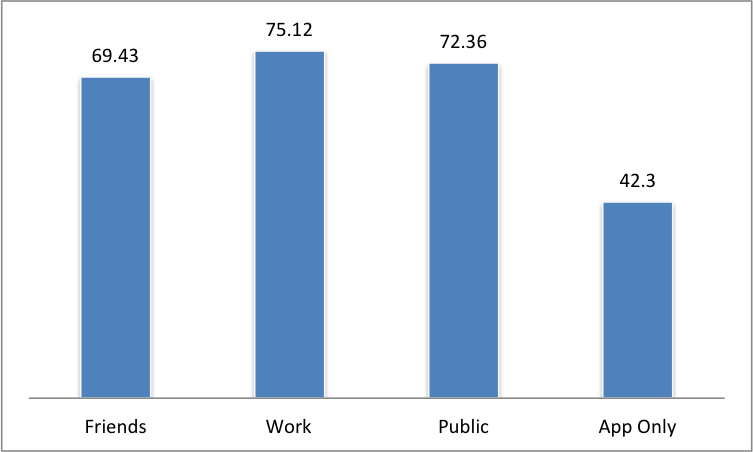
\includegraphics[width=0.5\textwidth]{recipient.png}
	\caption{(This is a placeholder! TODO: generate a better plot for data recipient)}
\end{figure}

\subsubsection{Device Type}


\begin{figure}
	\centering
	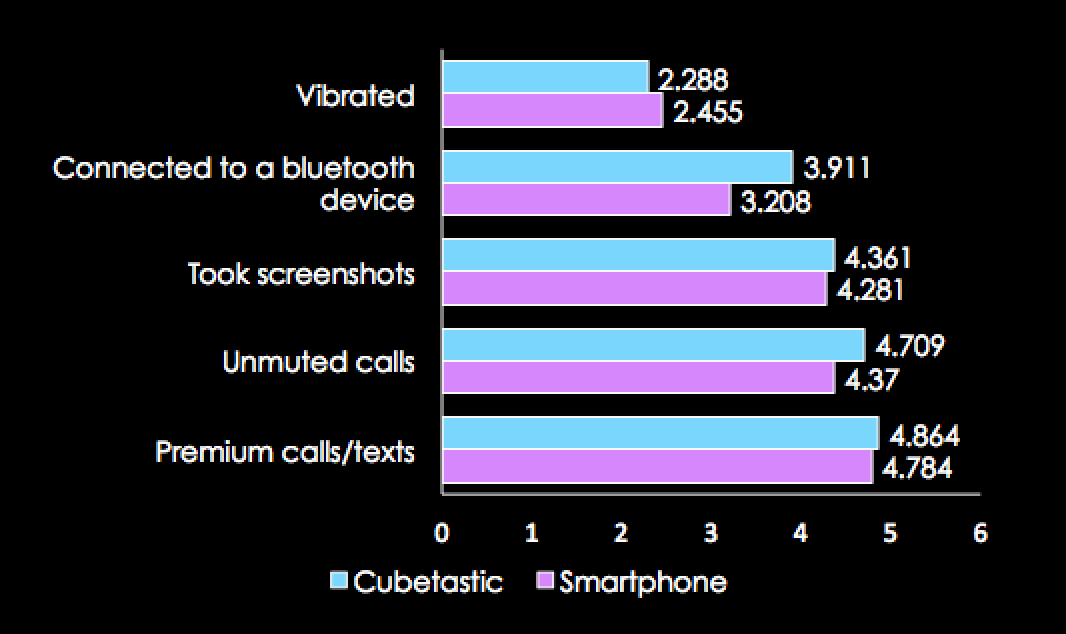
\includegraphics[width=0.5\textwidth]{device-type.png}
	\caption{(This is a placeholder! TODO: generate a better version of this)}
\end{figure}

\subsubsection{What Matters in Upsetting People}
(REDO) Talk about the regression model here. Say that the data type was x\% responsible, the data recepient y\% responsible, and the device type z\% responsible for how upset people seemed to be when they answered the questions. 

Also go into any correlations that I found with respect to demographics and the IUIPC index (I should do all of these things ASAP as soon as this paper is in good shape). There should be some interesting stuff there, whether there are specific correlations, or whether there is not. Both are good things to report and should be put here. 

\subsection{A Bigger Picture}

We asked users to rate how beneficial or risky a technology was, for all parties affected by the technology (including manufacturers, consumers, and bystanders), over a long period of time, with respect to other, well studied technologies. This gives us an interesting insight into how people perceive these new technologies. For instance, the capacity for facial detection on a wearable device is perceived to be as risky as interacting with a physical lawnmower. 

\begin{figure}
	\centering
	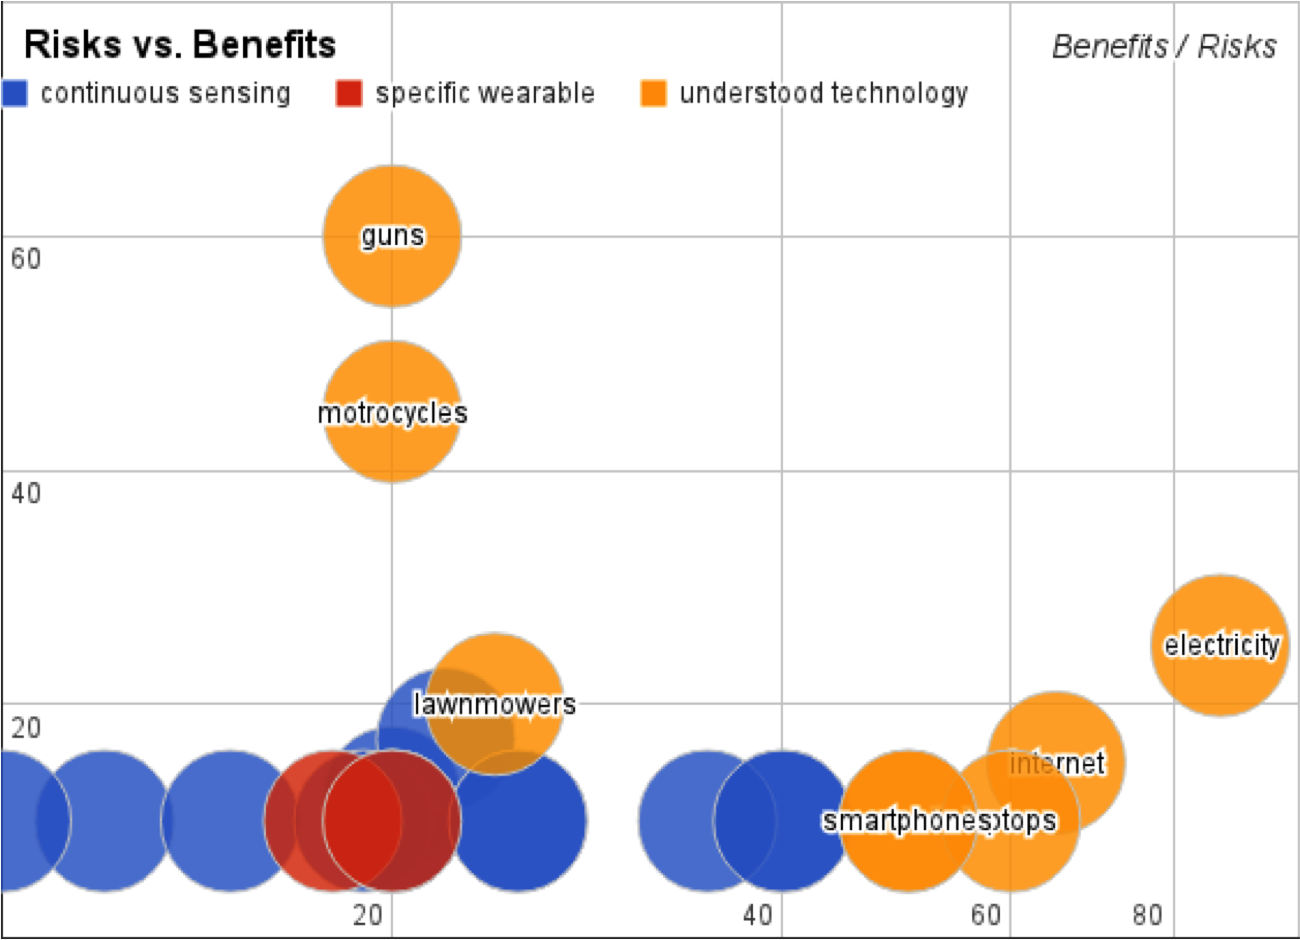
\includegraphics[width=0.5\textwidth]{techplot.png}
	\caption{(This is a placeholder! TODO: generate a better plot; take out the specific wearables too.)}
\end{figure}

\subsubsection{Risk and Benefit Ranks} 
(REDO) Talk through the graph shown above. The basic takeaway is that all of the new technologies and capabilities are perceived to be low risk low benefit. We can see that for technologies that people are more familiar with, people rate it more beneficial and more risky (or is it because they are more relevant that they are more familiar to them? Can I make such a claim?). Interesting to note facial recognition versus detection, location tracking, and discrete camera. Refer to appendix \ref{sec:techrank} for the details (if I have space to include such a thing as the absolute benefit and risk ranking and quartiles in this paper..). 

\subsubsection{Lawnmower Ratios} 
(REDO) The basic idea for this is that I am going to compare all of the newly assessed technologies with respect to the well-studied technology generally considered to be low-risk and low-benefit, since all new technologies fit this mold. This can give a more accurate idea into how each person thought something was risky or not (twice as risky as the closest tech they know, or about equal, etc.). Do some fancy graphing stuff here. Maybe another scatter plot, or an overlay of various distributions of ratio of perceived lawnmower risk to technology risk. Hmm. 

\subsection{Perceived Concerns for Wearable Devices}
(REDO) Although we asked users about particular situations which might occur with a wearable device and asked them to assess technologies in a general sense, our open ended question asked the users to state the most likely risk(s) associated with owning and interacting with wearable devices. Without any doubt, the most common concern for owning and interacting with wearable devices for the every day user is the \textit{loss of privacy}. 

(I should probably make a table of the following. Ugh, but for now:)

Privacy 				464 (25.99\%) \\
Security 				94 (5.27\%)\\
Hacking 				38 (2.13\%)\\
Spying 				50 (2.80\%)\\ [-.5cm]

Unaware Use 			167 (9.36\%)\\
Accidental Sharing 		66 (3.70\%)\\
Unaware Collection		64 (3.59\%)\\
Unaware Access	 	44 (2.46\%)\\
False Information 		33 (1.85\%)\\[-.5cm]

Health Risk 			252 (14.12\%)\\
Safety 				147 (8.24\%)\\
Financial Cost	 		201 (11.26\%)\\[-.5cm]

Social Impact 			135 (7.56\%)\\
Social Stigma 			39 (2.18\%)\\
Aesthetics 			19 (1.06\%)\\[-.5cm]

Miscellaneous 		76 (4.26\%)\\
None				51 (2.86\%)\\
Don't know			 30 (1.68\%)\\
Don't care 			6 (0.34\%)\\

Talk about the coding labels and what they mean, in a very vague and compact way. Refer people to the appendix \ref{sec:coding} for what the coding means in detail. 

Takeaway is that people care about privacy, then security, health, social impact. Other interesting things to note are aesthetics, social stigma, and false information, which could be cool things to look into. 

%%%%%%%%%%%%%%%%%%%

\section{Discussion}
We take this section to discuss complementary future research directions in fields of privacy, ubiquitous computing, and user studies, along with specific limitations of this survey. 

\subsection{Future Research Directions}
(REDO, ask David's/Serge's input for this section) Additional future work is encouraged in the area of studying privacy with respect to ubiquitous computing, since we proved it was the number one concern of the users of wearable devices. Clearly, this is a hard question which has been worked on for a long time but not yet fully addressed. Even this survey just barely touched on the various factors which can influence privacy perceptions and how upset people would be. 

 Also, maybe some work with respect to security threats, and how feasible they might be, and some defenses against stopping wearables devices from getting sensitive information (like blocking text, detecting sensitive situations like the bathroom, etc.). Research which defends against false information, false positive commands, and just more safeguards against the new system for wearables, whatever that is, is also something to really look into. 
 
 Work making sure that people are aware of what is going on, using indicators, not-too-transparent interfaces, and maybe being polite (recording rules follow social rules--think polite glass talk from Jaeyeon at MSR) are going to be valuable as wearables get more sophisticated but also more adopted by people. Think about it--put people in control of the technology, not technology shifting the social norms (our survey says that one of the top concerns of people were about how wearables will change social norms). 

\subsection{Limitations}
One of the main limitations of this work is that our participants might not have interest, or an accurate idea, of wearable devices and their capabilities. 83\% of our participants reported that they do not own a wearable device, but at this time, about ~15\% of the general population own and use wearable devices \cite{Nilsen}\cite{WearableStatNews}, so our study is reflective of the status quo. We believed that getting a representative survey base was a useful endeavor, although we could have easily recruited only wearable device owners or people specifically interested in wearables. However, that will also have its own bias and limitations as well, since they would not reflect the general population. We expect user perceptions to change as rapidly as wearable technologies and the rate of adoption change. 

Crowdourcing user studies in Mechanical Turk has its challenges \cite{kittur2008crowdsourcing}. While the Amazon Mechanical Turk population is diverse across several significant demographic dimensions such as age, gender, and income, it is not a precise representation of the U.S. population \cite{ross2010crowdworkers}\cite{kelley2010conducting}. Additionally, Amazon Mechanical Turk workers generally put a higher value on anonymity and hiding information, were more likely to do so, had more privacy concerns than the larger U.S. public \cite{kang2014privacy}. 

The survey was constructed in a way to randomize the order of the particular sets of questions participants saw, except for the open-ended question, which was always near the end of the survey, asked along with the demographics. For this reason, people were heavily primed for the open-ended question. However, this question was always shown before the IUIPC questions, so our results on privacy being the top concern isn't because of the bias from the privacy index. The intent of the open-ended question  was more to get a sense of what people were concerned of, and we believe the results do reflect their actual concerns, but with a bit more clarity, since the participants were already thinking about such risks related to wearables. 

(REDO, Should I even say this?) I messed up that motorcycle question. I wish I actually had a calibration point for high risk high benefit for the Fischoff technology assessment questions. But well, none of the new technologies fit that description so we didn't really need it critically. 

%%%%%%%%%%%%%%%%%%%

\section{Conclusion}
(REDO) END STRONG! Should I put this before the Discussion?  Echo the introduction a little, remind the people of the takeaways in a way that highlights the contribution of this paper. Intro: ``we studied user perceptions for threats in wearable devices, along with user perceptions of risk and benefit for emerging technologies and what they thought was the biggest risk for using wearable devices. Data type, data recipient, and device type all matter different amounts. All new technologies were perceived to be low risk low benefit but we think this is because people are unfamiliar with these technologies. Privacy was the number one concern, followed by security, then health, money, social norms changing and social stigma. Fantastic ending sentence here.''

I can talk about the results a little bit more in depth because people have already supposedly read my whole paper now. Pull out the subtleties I couldn't have done in the introduction, and go into specific details, shooting out numbers and statistics. Then conclude the whole thing with an inspirational pitch on how there is much future work to be done in this area, how this area is exciting, and how I basically helped people see both of these things. 

%\end{document}  % This is where a 'short' article might terminate

%ACKNOWLEDGMENTS are optional
\section{Acknowledgments}
NSF funding, SCRUB, BLUES. Also any people who helped.


%%%%%%%%%%%%%%%%%%%
%%%            BIB & ACKS          %%%
%%%%%%%%%%%%%%%%%%%

% The following two commands are all you need in the initial runs of your .tex file to produce the bib
%  and remember to run: latex bibtex latex latex to resolve all references

\bibliographystyle{abbrv}
\bibliography{wearables_survey}  % wearables_survey.bib is the name of the Bibliography


%APPENDICES are optional
%\balancecolumns
\appendix
%Appendix A
\section{Focus Group Script}
\label{sec:script}

text text

\section{Fischoff Prompts}
\label{sec:prompt}

text text 

\section{Risk and Benefit Rankings}
\label{sec:techrank}

text text

\section{Coding Label Definitions}
\label{sec:coding}

text text
%\section{Detailed Tech Rankings}

\balancecolumns

% That's all folks!
\end{document}
